
%-----------------------------------------------------------------------------
%	PACKAGES AND THEMES
%-----------------------------------------------------------------------------
\documentclass[ignorenonframetext]{beamer}


\usepackage[beamer]{shortcut}
\usepackage{ulem}

\graphicspath{{images/}}
\def\TikzLocation{./tikz/}
\def\tkzscl{1}


\setbeamertemplate{bibliography item}{}
\setbeamertemplate{bibliography entry title}{}
\setbeamertemplate{bibliography entry location}{}
\setbeamertemplate{bibliography entry note}{}
\bibliographystyle{apalike}


\hypersetup{
	colorlinks=true,
	urlcolor=linkcolor,
}


\AtBeginSection[]
{
 \begin{frame}<beamer>
 \frametitle{Plan}
 \tableofcontents[currentsection]
 \end{frame}
}

%-----------------------------------------------------------------------------
%	CUSTOM COMANDS
%-----------------------------------------------------------------------------

\def\keypoint#1{\hfill\textcolor{gray}{#1}}
\def\mycite#1{\keypoint{\cite{#1}}}




%----------------------------------------------------------------------------------------
%	PRESENTATION INFO
%----------------------------------------------------------------------------------------

\title[Neural Sparse Coding]{Understanding Trainable Sparse Coding with Matrix Factorization}

% Presentation info
\author{Thomas Moreau} % Your name
\institute[CMLA]{CMLA - ENS Paris-Saclay} 
\date{06/11/17} % Date, can be changed to a custom date

% Custom footline
\event{Tech talk}
\location{Google, Zurich}

% Logo Joan
\def\extraLogo{
  \includeLogos[1em]{logo_NYU,logo_UCB}
}

% Add collaborators
\collaborators[]{J. Bruna, J. Audiffren}
% ou
%\collaborators[collab]{Joan Bruna}

% Add supervisor
%\collaborators[supervised]{J. Doe, J. Smith}

% Title for a single frame
% The box around the title can be adapted with the \SizeTitleBox option
\setbeamertemplate{title page}[frame]
\setlength\SizeTitleBox{.8\textwidth}

% Title in a header for the first slide
%\setbeamertemplate{title page}[header]

%-----------------------------------------------------------------------------
%	DOCUMENT
%-----------------------------------------------------------------------------
\begin{document} 


%% Title page
{\setbeamertemplate{footline}{} 
\begin{frame}[t,plain]

	\titlepage

\end{frame}}


\begin{frame}<beamer>
 \frametitle{Plan}
 \tableofcontents
\end{frame}


\section{Physiological signals}



% Physiological signals ECG
\begin{frame}{Physiological signals}

	\centering
	\Large\textbf{ECG}\\[1em]
	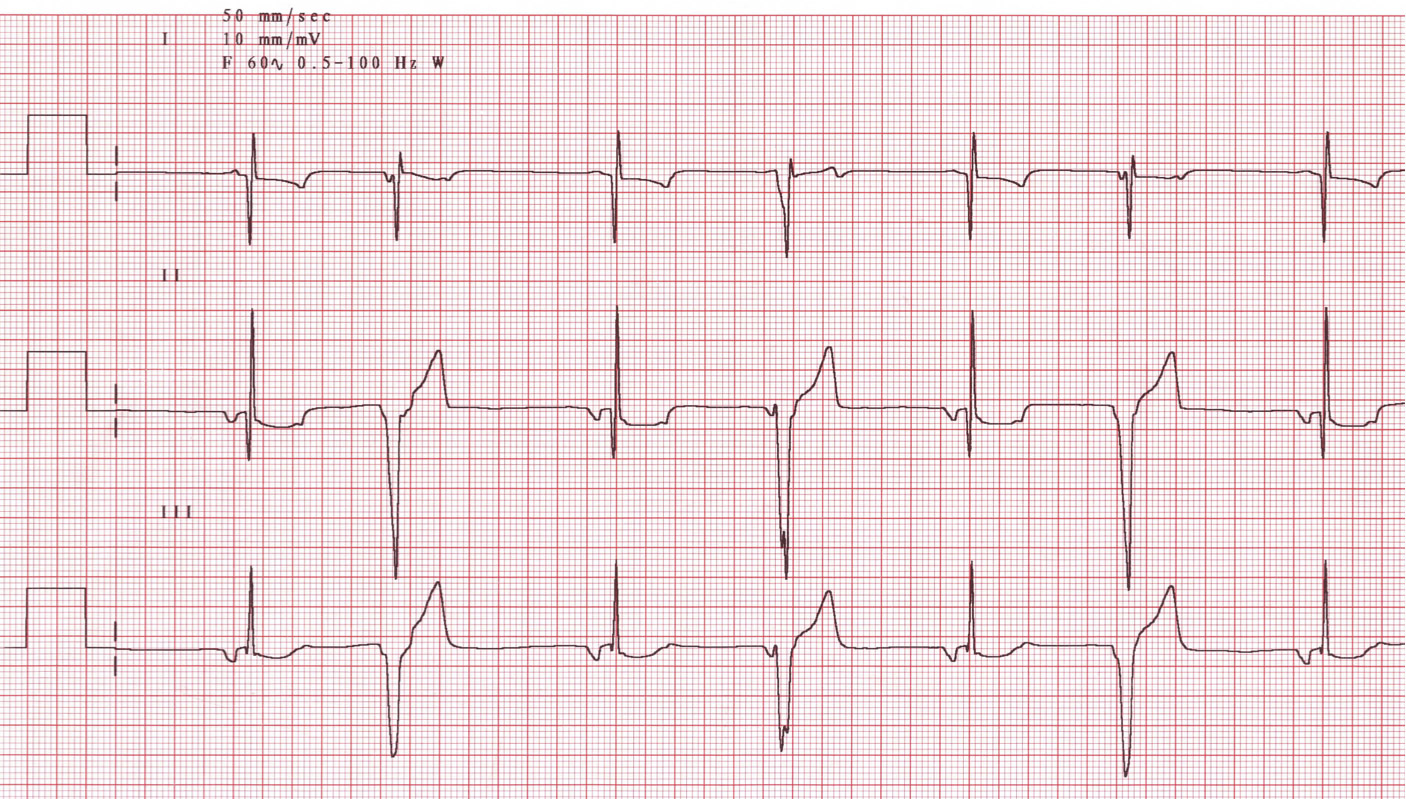
\includegraphics[width=.8\textwidth, height=7em, trim={0 0 0 2em}, clip]{ecg}
	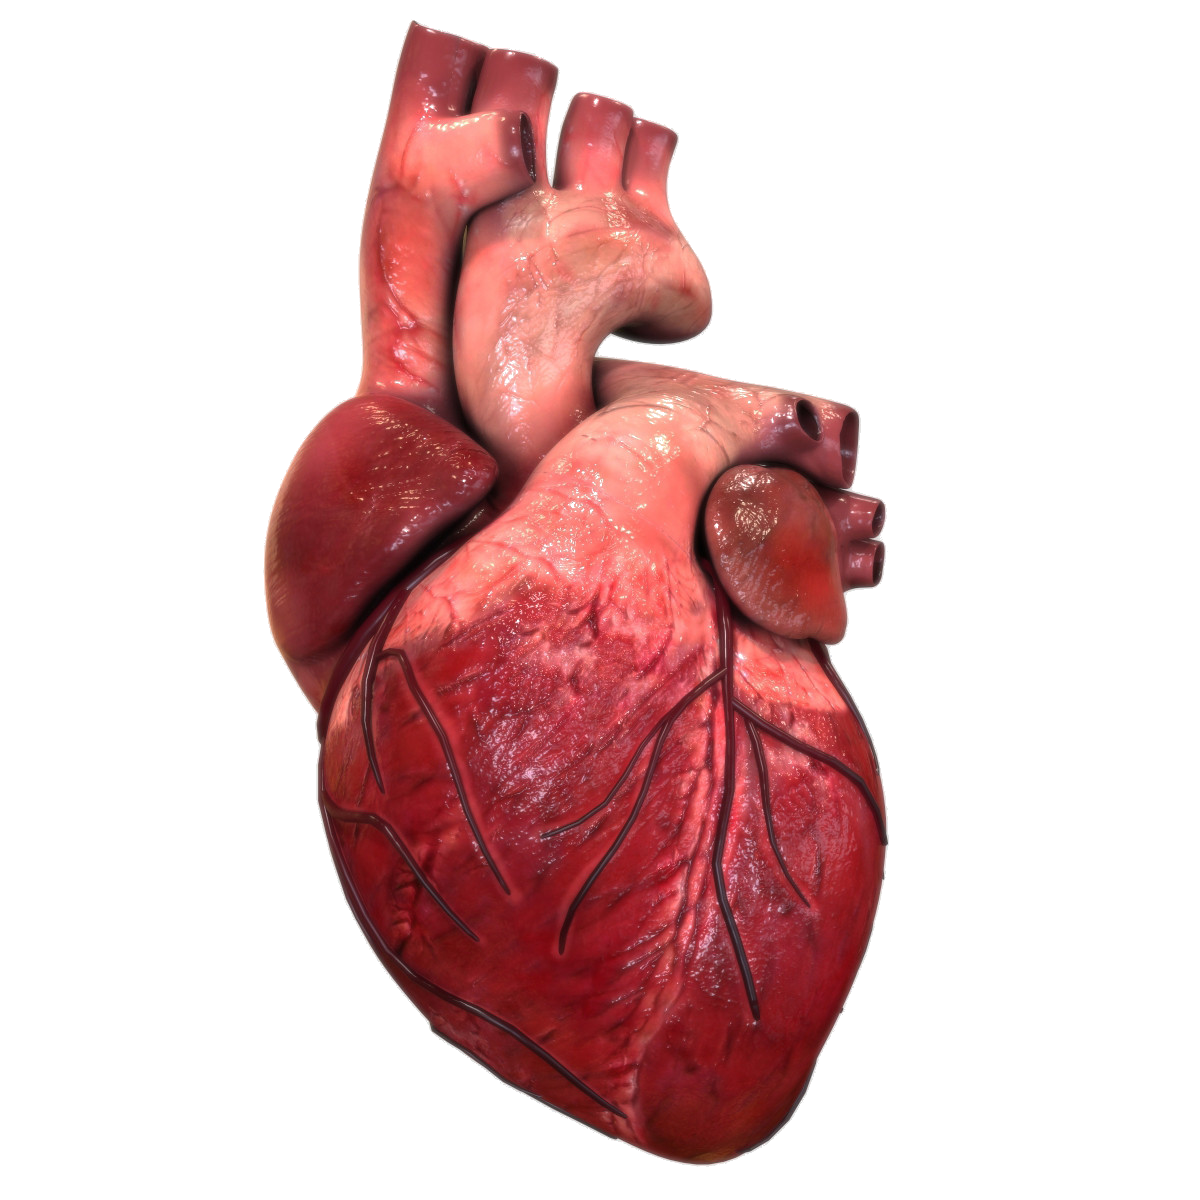
\includegraphics[width=.25\textwidth]{heart}\hskip2em
	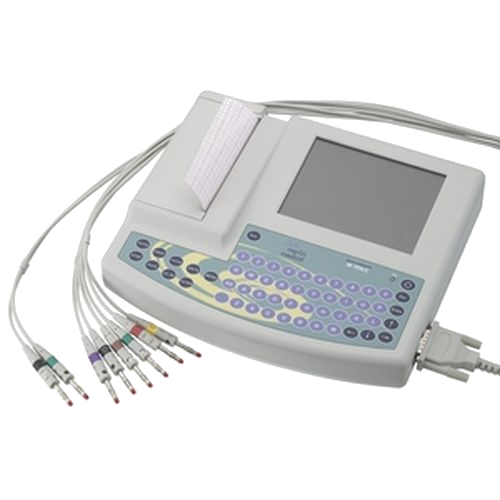
\includegraphics[width=.3\textwidth]{captor_ecg}

\end{frame}


% Physiological signals EEG
\begin{frame}{Physiological signals}

	\centering
	\Large\textbf{EEG}\\[1em]
	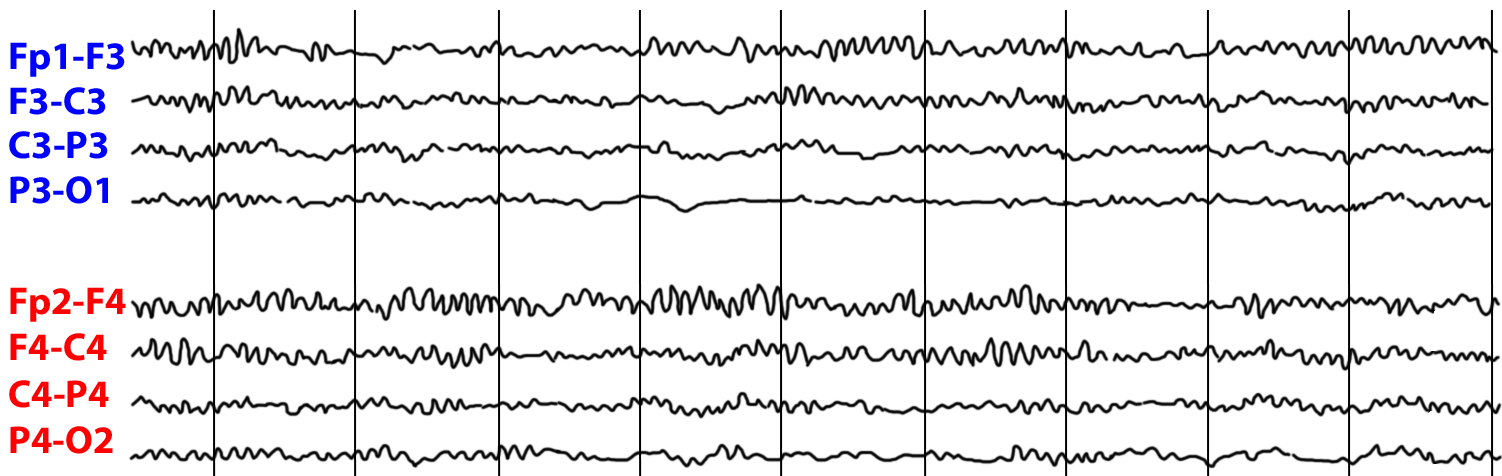
\includegraphics[width=.8\textwidth]{eeg_alpha}\\[.5em]
	
\includegraphics[width=.3\textwidth]{brain}\hskip2em
	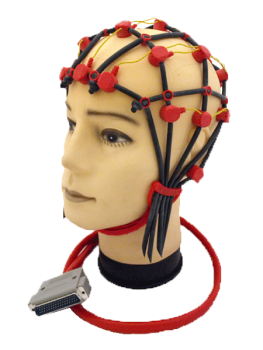
\includegraphics[width=.2\textwidth]{captor_eeg}

\end{frame}






% Physiological signals Oculo
\begin{frame}{Physiological signals}

	\centering
	\Large\textbf{Oculometric signals}\\[.5em]
	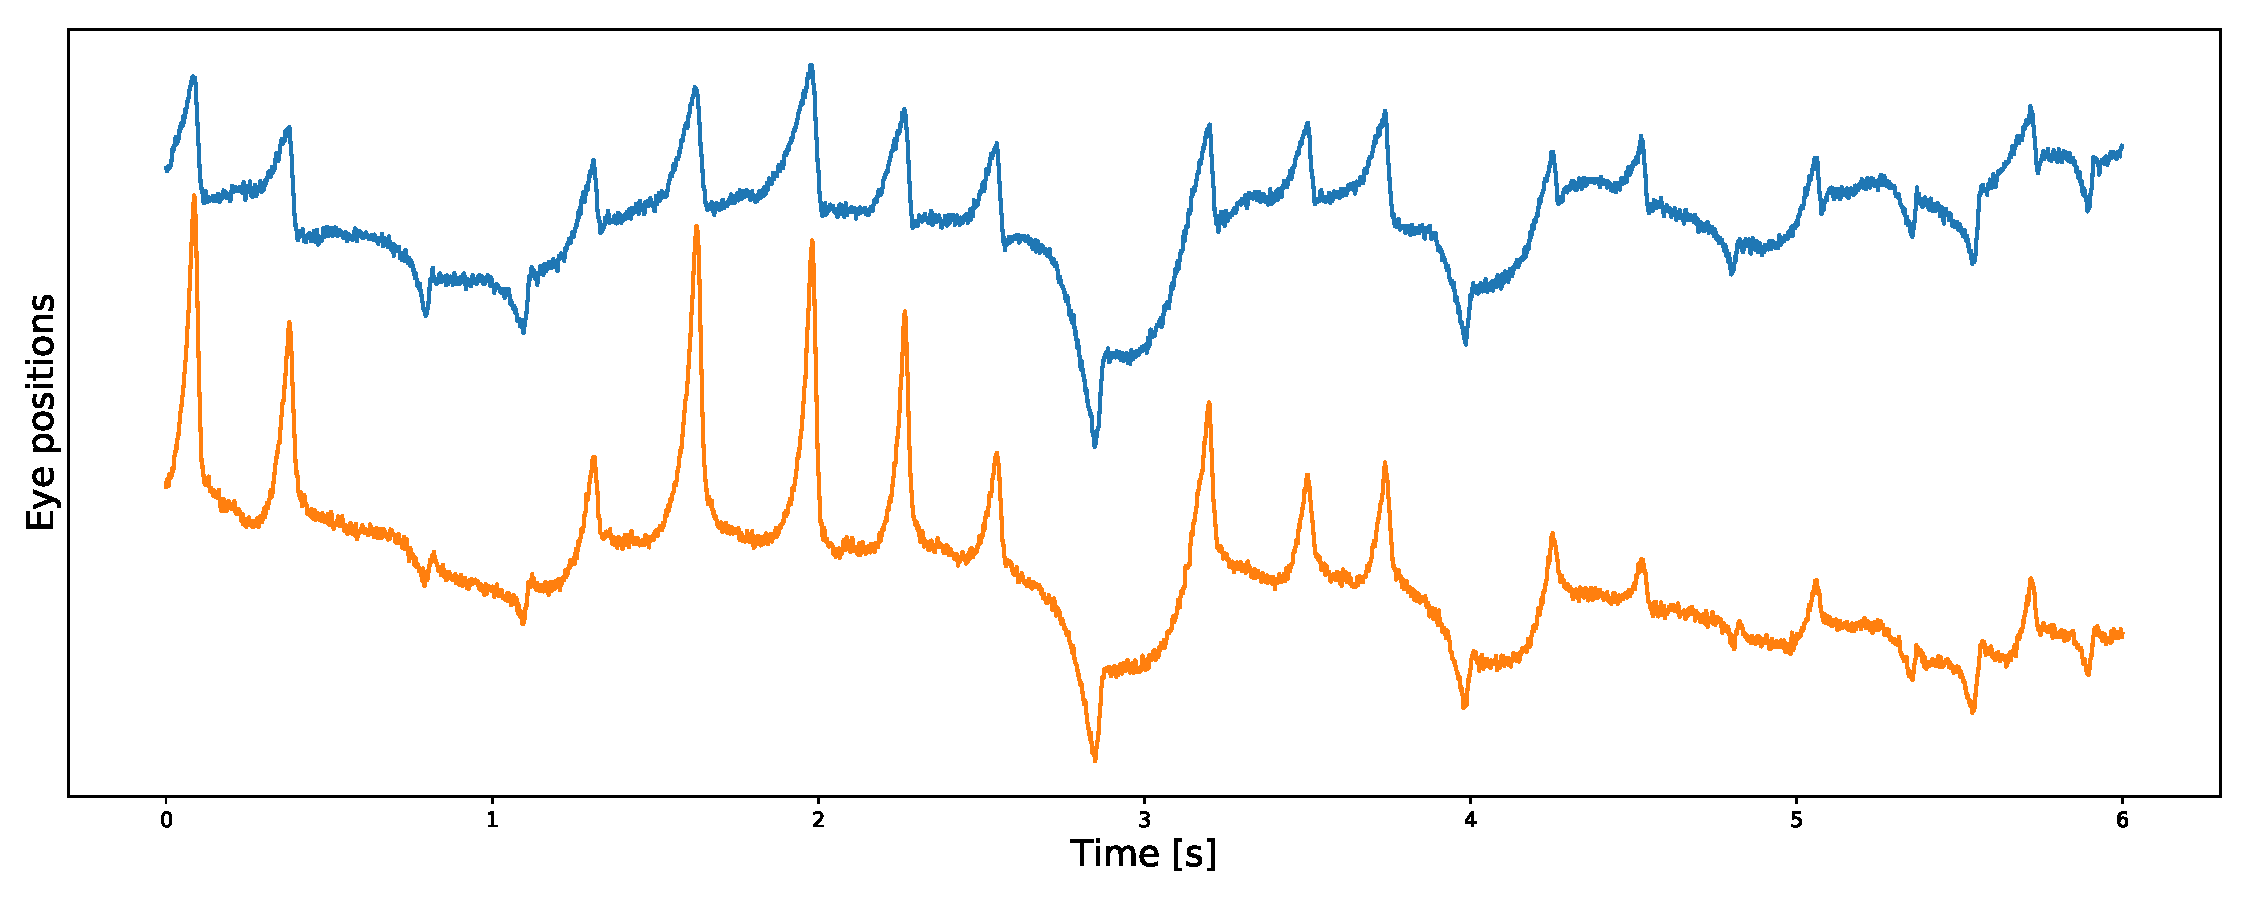
\includegraphics[width=.8\textwidth, height=7em]{oculo}\\[.5em]
	
\includegraphics[width=.25\textwidth]{eye}\hskip2em
	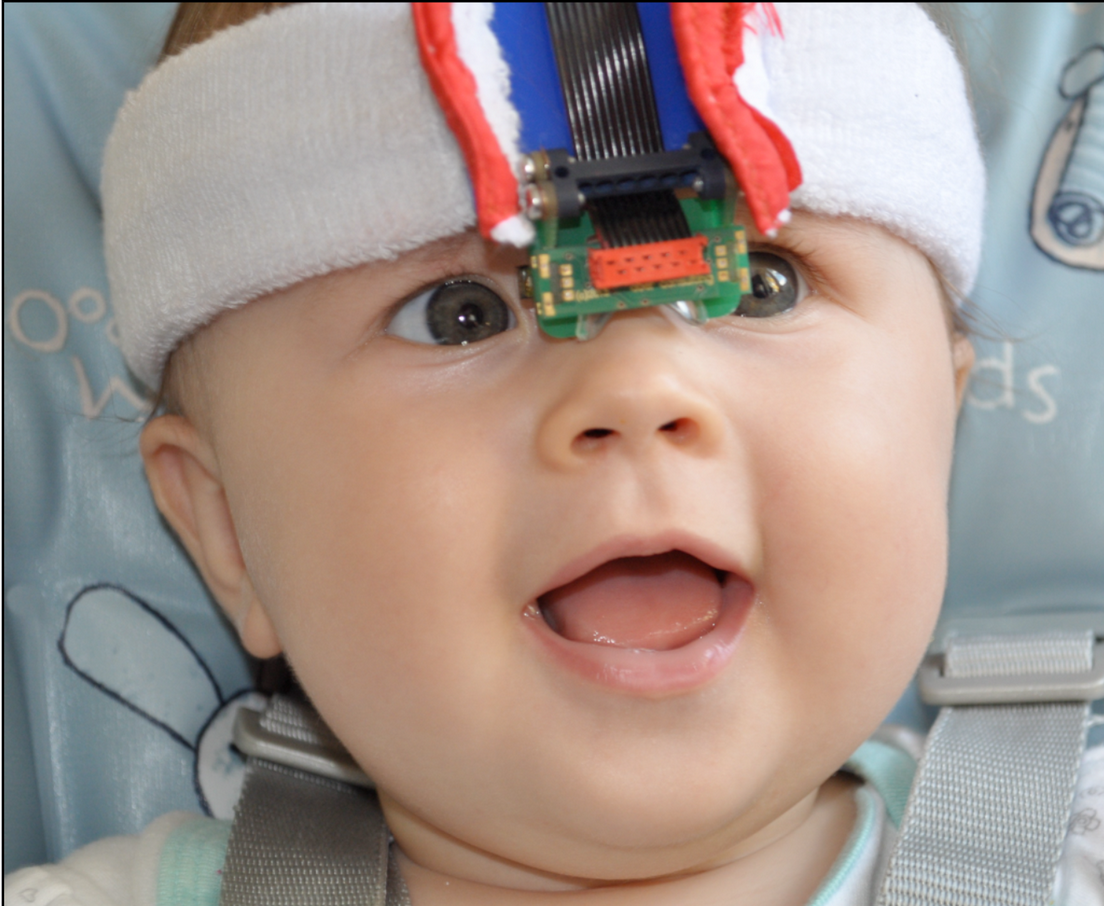
\includegraphics[width=.3\textwidth]{captor_ober}

\end{frame}



% Physiological signals Walk
\begin{frame}{Physiological signals}

	\centering
	\Large\textbf{Accelerometers}\\[1em]
	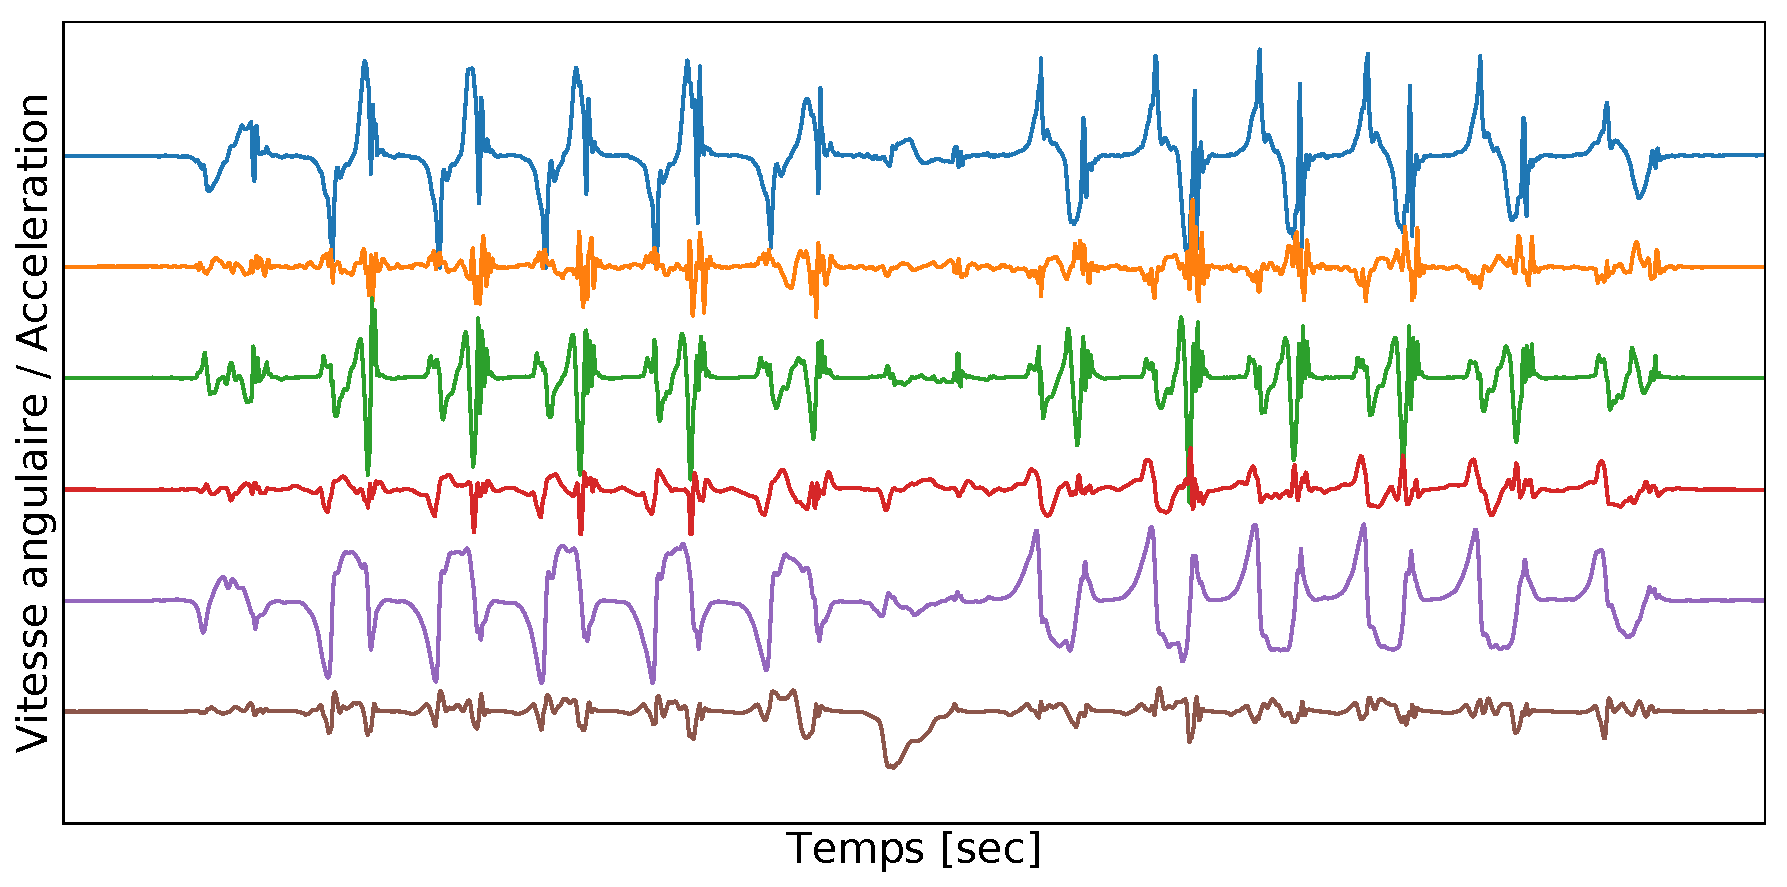
\includegraphics[width=.8\textwidth, height=7em]{accelero}\\[.5em]
	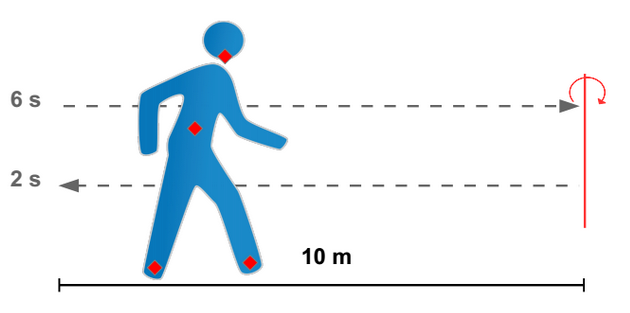
\includegraphics[width=.4\textwidth]{exo_marche}\hskip2em
	\raisebox{2.5em}{\Large $4\times$} 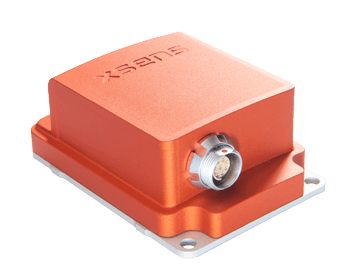
\includegraphics[width=.3\textwidth]{xsens}

\end{frame}

% Statistical tools for signal analysis
\begin{frame}{Statistical analysis for Time Series}
\setbeamercovered{transparent}
\Large

	\begin{itemize}\itemsep1em
		\item Failure of the vectorial distances\\[.5em]
		\begin{itemize}\itemsep1em\itemindent0em\large
		\item Alignment issues, different lengths\\\keypoint{(can be solved with DTW)}
		\item "Curse of dimensionality"
	\end{itemize}
		\item Different approaches which can be classified in 2 categories:\\[.5em]
	\begin{itemize}[<1>]\itemsep1em\large
		\item Model based methods:\\\hskip1em feature extraction + vectorial method, \dots
		\item <-2>{Data driven methods\\\hskip1em End-to-end model, Neural networks, \dots}
	\end{itemize}
	\end{itemize}

\end{frame}


\section{End-to-end Approaches for Time Series}


\begin{frame}{End-to-end Approaches}
\Large
{\bf Neural Networks:\\[.3em]}
	\begin{itemize}\itemindent2em\itemsep.25em
		\item Raw signal as input, \\[.25em]
		\keypoint{No feature-engineering}
		\item Internally select the data representation,\\[.25em]
		\keypoint{Adaptive}
		\item Representation adapted to the task,\\[.25em]
		\keypoint{Performant}
		\item Simple training algorithms, \\[.25em]
		\keypoint{Scalable}
	\end{itemize}

\end{frame}


\begin{frame}{Theoretical guarantees}
\Large
	{\bf Split between risk error 3 terms: }\\\mycite{Bottou2008}\\[1em]
	\begin{itemize}\itemsep.3em\itemindent2em
	\item Approximation error: Universal approximation,
	\\[.25em]\mycite{Hornik1991}
	\item Estimation error: Generalization bound,
	\\[.25em]\mycite{Neyshabur2017}
	\item Optimization error: Learning convexification,
	\\[.25em]\mycite{Haeffele2017}
\end{itemize}

\end{frame}

\begin{frame}{Neural Networks}

	\centering \Large
	{\bf Main drawback: }\\[1em]
	Lack of interpretability. It is often seen as a black box.\\[2em]
	
	How can we bring interpretability in the internal representation?

\end{frame}

\begin{frame}{End-to-end Approaches}
\Large
{\bf Task-driven Dictionary Learning:}\\\mycite{Mairal2012}\\[.3em]
	\begin{itemize}\itemindent2em\itemsep.25em
		\item Raw signal as input, \\[.25em]
		\keypoint{No feature-engineering}
		\item Representation adapted to the task,\\[.25em]
		\keypoint{Performant}
		\item Complex training algorithms, \\[.25em]
		\keypoint{\sout{Scalable}}
		\item Highlight local structures,\\[.25em]
		\keypoint{Interpretable}
	\end{itemize}

\end{frame}


\begin{frame}{Problematic}

	\centering \huge
	{\bf Can we study the links between these two models to bring more interpretability in neural networks?}

\end{frame}

\section{Post-training for Deep Learning}
\label{sec:post_train}


\begin{frame}{Post-training for Deep Learning}

	{\bf Paper with J. Audiffren: } arxiv:1611.04499\\[2em]

	Use the idea to split the representation learning and the task resolution:\\[1em]
	\begin{itemize}\itemindent1em\itemsep1.5em
		\item \underline{{\it Post-training} step:} only train the last layer,
		\item \underline{Easy problem:} this problem is often convex,
		\item \underline{Link with kernel:} close form solution for optimal last layer.
		\item \underline{Experiments:} consistent performance boost with multiple architecture.
	\end{itemize}
	
\end{frame}

% section post_train (end)


\section{Adaptive Iterative Soft Thresholding}
\label{sec:adapt}


\begin{frame}{LASSO \hfill\hfill\hfill\hfill\hfill \mycite{Tibshirani1996}}
	The LASSO or sparse coding problem is defined as
	
	\begin{equation}
        \label{eq:lasso}
        \argmin_z F(z) := \underbrace{\|x - Dz\|_ 2^2}_{E(z)} + \lambda\|z\|_1~,
	\end{equation}
	
	where $x \in \mathbb R^P$, $D \in \mathbb R^{P\times K}$ and $z \in \mathbb R^K$.\\[2em]

	
	(\autoref{eq:lasso}) can be rewritten as a proximal problem for the $B$-norm
	\[
	\argmin_z \underbrace{(y-z)\tran B (y-z) }_{E(z)} + \lambda \|z\|_1
				\hspace{1em}{\color{gray}\left(= F(z)\right)}
	\]
	where $B = D\tran D$ is the Gram matrix of $D$ and $y = D^\dagger x$.\\[.5em]
\end{frame}

\begin{frame}{Learned ISTA \hfill\hfill\hfill\hfill\hfill \mycite{Gregor10}}


	Accelerate the LASSO resolution using a neural network.\\[1em]

	\begin{figure}
	\begin{subfigure}[b]{.47\textwidth}
		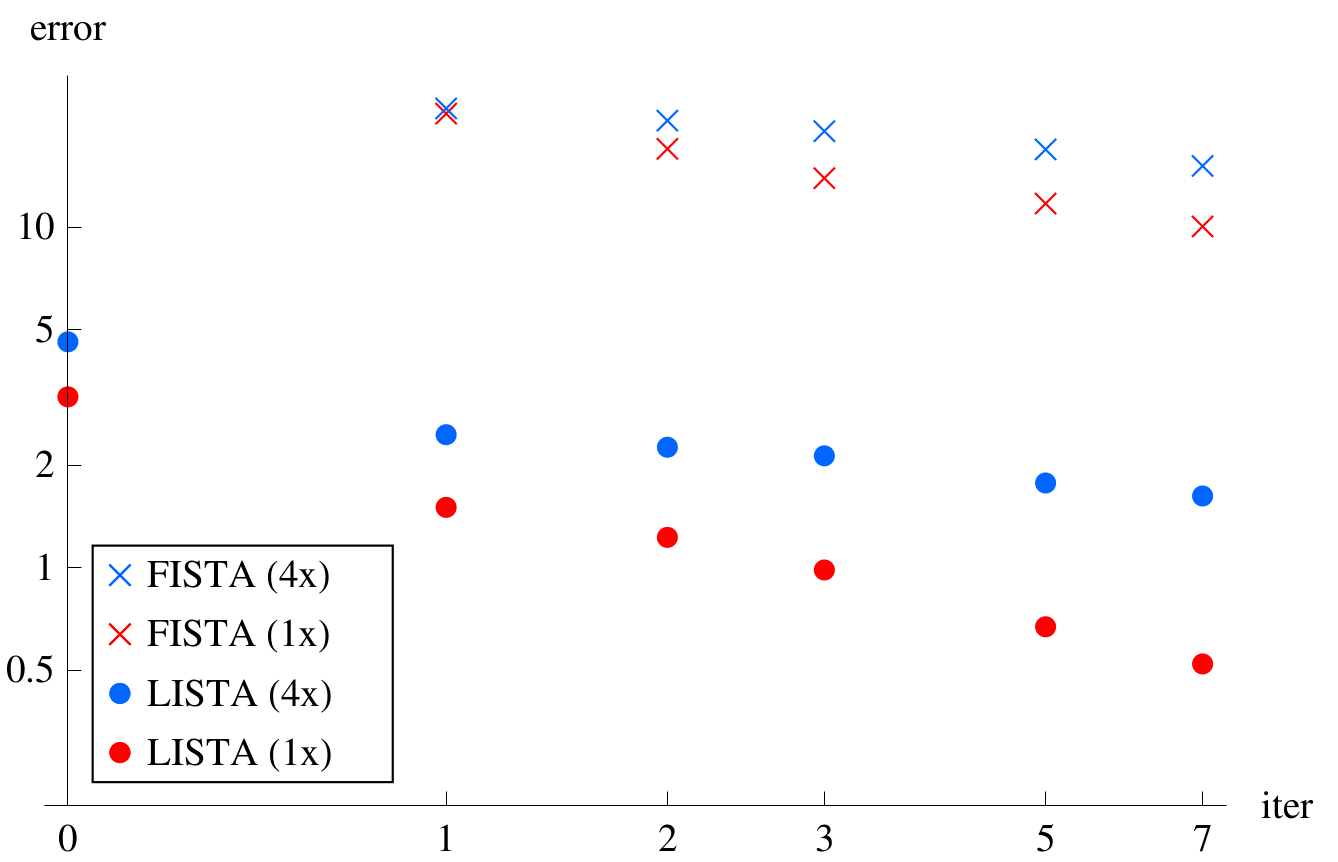
\includegraphics[width=\textwidth]{Gregor10}
	\end{subfigure}
	\begin{subfigure}[b]{.5\textwidth}
		\centering
		\inputTikZ{.8}{ista_tikz.tex}
		\inputTikZ{.6}{lista_tikz.tex}
	\end{subfigure}
	\caption{Adapted from \cite{Gregor10}}
	\end{figure}
	\vskip1em

	Link dictionary learning model and sparse representation.\\[2em]

	\centering
	\textbf{Why does it work?}
\end{frame}


%\begin{frame}{Dictionary Learning}
%\includegraphics[width=.47\textwidth]{dictionary_learning}
%\includegraphics[width=.47\textwidth]{dictionary_learning_noise}
%\end{frame}

\begin{frame}{ISTA (1/2) \hfill\hfill\hfill\hfill\hfill \mycite{Daubechies2004,Beck2009}}


	Surrogate function $F_q$ associated with point $z^{(q)}$ :
	\[
		F_q(z) = E(z^{(q)}) + \langle B(z^{(q)}-y) , z-z^{(q)} \rangle
				+ \frac{\|B\|_2}{2}\| z - z^{(q)} \|_2^2 + \lambda \|z\|_1~,
	\]

	\begin{block}{Properties}
	\vskip.5em
		This surrogate function satisfies
		\begin{enumerate}
		    \item $F_q(z^{(q)}) = F(z^{(q)})$
			\item for all $z$, $F_q(z) \geq F(z) $,
			\item solving $\argmin_z F_q(z)$ is computationally efficient.
		\end{enumerate}
	\end{block}
\end{frame}

%\begin{frame}[t,noframenumbering]{ISTA (1/2)}
%\begin{columns}
%    \column{.49\textwidth}
%	    \centering
%	    \includegraphics[width=\textwidth]{cost_fun1}\\
%	    Quadratic form $z\tran Bz$
%    \column{.49\textwidth}
%	    \centering
%	    \includegraphics[width=\textwidth]{cost_fun2}\\
%	    Replace $B$ with $\frac{L}{2} \pmb I_K$
%\end{columns}
%\end{frame}

\begin{frame}{ISTA (2/2)}
\begin{columns}[T]
	\hskip.03\textwidth
	\column{.55\textwidth}
	\underline{Iterative procedure:} \keypoint{proximal splitting}
	\begin{equation}
		\begin{aligned}
		    z^{(q+1)} &= \argmin_z F_q(z)\\
		    &= \prox_{\lambda\|\cdot\|_1}\left(z^{(q)} - \frac{1}{L} \nabla E(z^{(q)})\right)
		\end{aligned}
		\label{eq:ista}
	\end{equation}

	\begin{block}{Properties}
		\vskip.5em
		\begin{enumerate}\itemsep.5em
			\item $z^*$ is a fix point of (\autoref{eq:ista}),
			\item Efficient computation for $z^{(q+1)}$ as the problem is separable,
			\item Convergence in $\mathcal O\left(\frac{1}{q}\right)$ in general.
		\end{enumerate}
	\end{block}


	\column{.5\textwidth}
	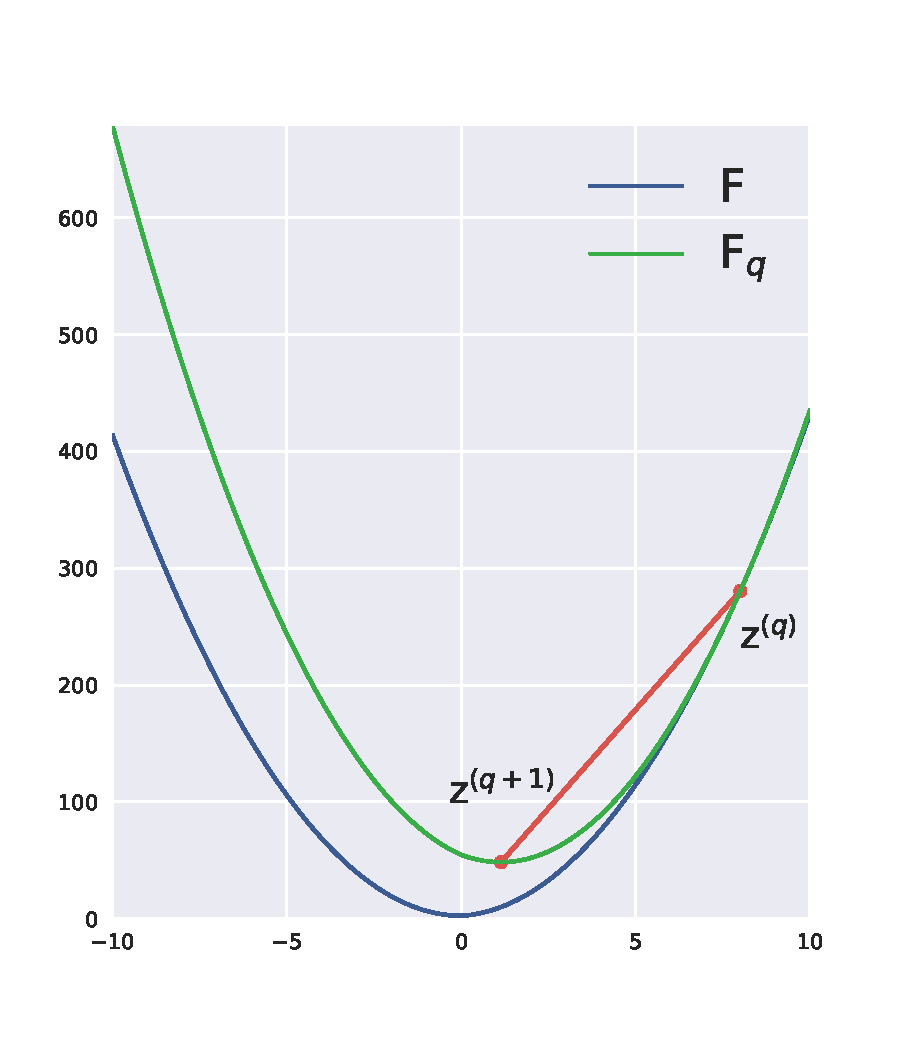
\includegraphics[width=\textwidth]{ista_step}


\end{columns}
\end{frame}


\begin{frame}{Why does it work?}

\begin{itemize}\itemsep2em

	\item \textbf{Guaranteed descent}\\[.8em]
	The construction of the next point guarantees the cost function is decreasing:
	\[
		F(z^{(q+1)}) \le F_q(z^{(q+1)}) \le F_q(z^{(q)}) = F(z^{(q)})
	\]

	\item \textbf{Efficient computation:}\\[.8em]
	With the isotropic quadratic form $\frac{L}{2}\pmb I_K$, the function $F_q$ is separable.\\[.3em]
	The computation are linear in $K~$.

\end{itemize}

\end{frame}


%\begin{frame}{Solving multiple optimization problems}

%\begin{itemize}\itemsep2em
%	\item Solve more than one instance of a problem:
%	\begin{itemize}
%		\item Regularization path \keypoint{(Multiple $\lambda$)}
%		\item Multi-objective regression \keypoint{(Multiple labels $x$)}
%		\item Sparse coding  \keypoint{(Multiple data points $x$)}
%		\item \dots
%	\end{itemize}
%	\item Regular optimization techniques does not leverage the common structure of these problems:
%	\begin{itemize}
%		\item Designed to solve the worst case,
%		\item Fix updates, without using information from previous resolutions.
%	\end{itemize}
%\end{itemize}

%\vskip1.5em
%Study the gain we can get by leveraging the structure of the set of problem.  
%Can we use the global structure of the problem to accelerate its resolution?
%\end{frame}


\begin{frame}{Toward an adaptive procedure}

	We define $Q_S(u, v) = \frac{1}{2}(u-v)\tran S (u-v) + \lambda \|u\|_1~.$\\[1em]
	\underline{\bf ISTA:}
	\begin{eqnarray*}
		F_q(z) & = & E(z^{(q)}) + \langle B(z^{(q)} - y) , z-z^{(q)} \rangle
						+ Q_{L\pmb I_K}(z, z^{(q)})~,\\
			   & \rightarrow & \min_z Q_{L\pmb I_K}(z, z^{(q)} - \frac{1}{L}B(z^{(q)} - y))
	\end{eqnarray*}
	\hskip3em{\Large $ \color{darkblue} \Rightarrow$} Replace $B$ with an upperbound $L\pmb I_K $\\[1em]
	\underline{\bf FacNet:} For any matrix $S$ diagonal, and $A$ unitary we define :
	\begin{eqnarray*}
		\widetilde F_q(z) & = &
					E(z^{(q)}) + \langle B(z^{(q)} - y) , z-z^{(q)} \rangle
						+ Q_S({\color{blue} A}z, {\color{blue} A}z^{(q)})~,\\
						& \rightarrow & \min_z Q_S(Az, Az^{(q)} - S^{-1}A B(z^{(q)} - y))
	\end{eqnarray*}
	\hskip3em
	{\Large $ \color{darkblue} \Rightarrow$}
	Replace $B$ with an approximation $A\tran SA$\\[1em]

	Can we choose $A, S$ to accelerate the optimization compared to ISTA? 

\end{frame}

\begin{frame}{Toward an adaptive procedure}
	

	Similar iterative procedure with steps adapted to the problem topology.\\[1em]
	\[
		\widetilde{F_q}(z) = F(z) + (z-z^{(q)})\tran R(z-z^{(q)}) + \delta_A(z)
	\]
%\textbf{Proximal resolution :}
%\[z^{(q+1)} = \argmin_z F(z) = E(z^{(q)}) + \langle B(z^{(q)}-y) , z-z^{(q)} \rangle + \frac{1}{2}\| z - z^{(q)} \|_B^2 + G(z)~ ,\]
%$\color{darkblue}\Rightarrow$ Not computationally efficient but quick minimization.\\[1.5em]


	Tradeoff between:\\[.3em]
	\begin{itemize}\itemsep1em
		\item Rotation to align the norm $\|\cdot\|_B$ and the norm $\|\cdot\|_1$~,
		\keypoint{Computation}
		\[ R = A\tran SA - B\]
		\item Deformation of the $\ell_1$-norm with the rotation $A$~.
		\keypoint{Accuracy}
		\[ \delta_A(z) = \lambda\left(\|Az\|_1-\|z\|_1\right) \]
	\end{itemize}
	
\end{frame}


\begin{frame}{One step improvement	}
	\begin{block}{Proposition}
		\label{bi1}
		Suppose that $R = A\tran S A - B \succ 0$ is positive definite, and define 
		\[z^{(q+1)} = \arg\min_z \widetilde{F_q}(z)~,\]
		Then
		\[
			F(z^{(q+1)}) - F(z^*) \leq \frac{1}{2}(z^{(q)} - z^*)\tran R (z^{(q)} - z^*)
									+ \delta_A(z^*) - \delta_A(z^{(q+1)})~.
		\]
	\end{block}
	\vskip3em
	We are interested in factorization $(A, S)$ for which $\|R\|_2$ and $\delta_A$  are small.
\end{frame}

\begin{frame}{Adaptive Iterative Soft thresholding - Convergence rate}

    \begin{block}{Theorem}
    Let $A_q, S_q$ be the pair of unitary and diagonal matrices corresponding to iteration $q$, 
chosen such that $R_q = A_q\tran S_q A_q - B \succ 0$.
It results that
{\small 
\begin{equation*}
\label{zo1}
%F(z_{k}) - F(z^*) \leq \frac{(z^*- z_0)\tran R_0 (z^* - z_0) + 2 |\delta_{A_0}(z_{1}) - \delta_{A_0}(z^*) | }{2k} + \frac{\alpha - \beta}{2k}~,\text{ with}
	\begin{split}
		F(z^{(q)}) - F(z^*) \leq &\frac{(z^*- z^{(0)})\tran R_0 (z^* - z^{(0)}) + 2 L_{A_0}(z^{(1)}) \|  (z^*-z^{(1)}) \|_2 }{2q}\\
			&\hskip3em + \frac{\alpha_q - \beta_q}{2q}~,
	\end{split}
\end{equation*}
%$$\alpha = \sum_{n=1}^{k-1} \left(  2| \delta_{A_n}(z_{n+1}) - \delta_{A_n}(z^*)| + (z^* - z_n)\tran ( R_{n-1} - R_{n}) (z^* - z_n) \right)~,$$
\[\alpha_q = \sum_{i=1}^{q-1} \left(  2L_{A_i}(z^{(i+1)})\|(z^*-z^{(i+1)}) \| + (z^* - z^{(i)})\tran ( R_{i-1} - R_{i}) (z^* - z^{(i)}) \right)~,\]
\[\beta_q = \sum_{i=0}^{q-1} (i+1)\left((z^{(i+1)}-z^{(i)})\tran R_i (z^{(i+1)}-z^{(i)}) + 2\delta_{A_i}(z^{(i+1)}) - 2\delta_{A_i}(z^{(i)}) \right)~,\]}
where $L_A(z)$ denote the local Lipschitz constant of $\delta_A$ at $z$.
    \end{block}
\end{frame}

\begin{frame}{Interpretation}

	\begin{itemize}\itemsep2em
		\item For $A_q = \pmb I_K$ and $S_q = \|B\|_2 \pmb I_K$, the procedure is
		equivalent to ISTA, with the same rate of convergence.
		\item If $\displaystyle\|R_0\|_2 + 2 \frac{L_{A_0}(z_1)}{\|z^*-z_0\|_2} \le \frac{\|B\|_2}{2}$
			  and $A_q = \pmb I_K$ and $S_q = \|B\|_2 \pmb I_K$ for $k >0$, then the procedure get a
			  head start compare to ISTA
		\item {\bf Phase transition :}\\
		The upper bound is improved when
		$\displaystyle\|R_q\|_2 + 2 \frac{L_{A_q}(z^{(q+1)})}{\|z^*-z^{(q)}\|_2} \le \frac{\|B\|_2}{2}$,
		it is thus harder to gain as $\|z^{(q)} - z^*\|_2 \to 0$
	\end{itemize}
	
\end{frame}

\begin{frame}{Generic Dictionaries}
	
	A dictionary $D \in \Rset^{p\times K}$ is a generic dictionary when its columns
	$D_i$ are drawn uniformly over the $\ell_2$ unit sphere $\mathcal S^{p-1}$.

	\begin{block}{Theorem (Acceleration conditions)}
		In \textbf{expectation over the generic dictionary} $D$, the factorization algorithm using a
		diagonally dominant matrix $A\subset\mathcal E_\delta$, has better performance for
		iteration $q+1$ than the normal ISTA iteration -- which uses the identity -- when
		\[
			\lambda\E[z]{\|z^{(q+1)}\|_1+\|z^*\|_1}
				\le \sqrt{\frac{K(K-1)}{p}} \underbrace{\E[z]{\|z^{(q)}-z^*\|_2^2}
				}_{\substack{\text{expected resolution}\\\text{at iteration $q$ }}}
		\]
	\end{block}
\end{frame}
\begin{frame}{Generic Dictionaries}

	\begin{block}{Corollary (Acceleration conditions)}
		
		If the input distribution and the regularization parameter $\lambda$  verify
		\[
			\frac{\lambda\sqrt{p}}{8} \le \E[z]{\|z^*\|_1}~,
		\]
		Then for any resolution $\E[z]{\|z^{(q)} - z^*\|_2} = \epsilon > 0$ at iteration
		$q$, the performance of our factorization algorithm is better than the
		performance of ISTA, in expectation over the generic dictionaries.
	\end{block}

	\vskip2em
	FacNet can improve the performances compared to ISTA when this is verified.
\end{frame}

\section{Numerical Experiments}


\begin{frame}{Learned ISTA \hfill\hfill\hfill\hfill\hfill \mycite{Gregor10}}
\begin{figure}[t]
	\centering
	\inputTikZ{1}{ista_tikz.tex}
	\inputTikZ{1}{lista_tikz.tex}
	\label{fig:ista}
	\caption{Network architecture for ISTA/LISTA. LISTA is the unfolded version of the RNN of ISTA, trainable with back-propagation.}
\end{figure}
If $W_e = \frac{D\tran}{L} $ and $W_g = I - \frac{B}{L}$, this network is exactly 2 iterations of ISTA.
\end{frame}

\begin{frame}{FacNet}
Specialization of LISTA
	\[
		z^{(q+1)} = A\tran \prox_{S}( Az^{(q)} - S^{-1}A B(z^{(q)} - y))~,
	\]
	with $A$ unitary and $S$ diagonal.\\
Same architecture with more constraints on the parameter space:
\begin{equation*}
\begin{cases}
	W_e & = S^{-1}A D\tran\\
	W_g & =  A\tran - S^{-1}A BA\tran
\end{cases}
\end{equation*}
\vskip1em
\hskip3em $\Rightarrow$ LISTA can be at least as good as this model.
\end{frame}

\begin{frame}{Learned FISTA}
The same ideas can also be applied to FISTA to obtain similar procedures:
\begin{figure}[t]
    \centering
	\inputTikZ{.75}{lifsta_tikz.tex}
    \label{fig:ista}
    \caption{Network architecture for L-FISTA.}
\end{figure}
\end{frame}


\begin{frame}{Artificial simulation}
   
   {\bf Generating Model: }\\
   \begin{itemize}\itemsep1em
	\item $D = \left(\frac{d_1}{\|d_1\|_2}, \dots \frac{d_K}{\|d_K\|_2}\right)$
	with $d_k \sim \mathcal N(0, \pmb I_P)$ for all $k\in \llbracket 1, K\rrbracket$~,
	\item $z = (z_1, \dots z_K)$ are constructed following a bernouilli gaussian:
	\[z_k = b_ka_k, \hskip2em b_k \sim \mathcal B(\rho) \text{ and } a \sim \mathcal N(0, \sigma \pmb I_K)\]
\end{itemize}
	
	\emph{with: } $K = 100$, $P = 64$, for the dimension, $\sigma = 10$ and $\lambda = 0.01$\\[2em]
	
	\hskip3em $\Rightarrow$ The sparsity patterns are uniformely distributed.
	
\end{frame}

\begin{frame}[noframenumbering]{Artificial simulation}
	\centering
    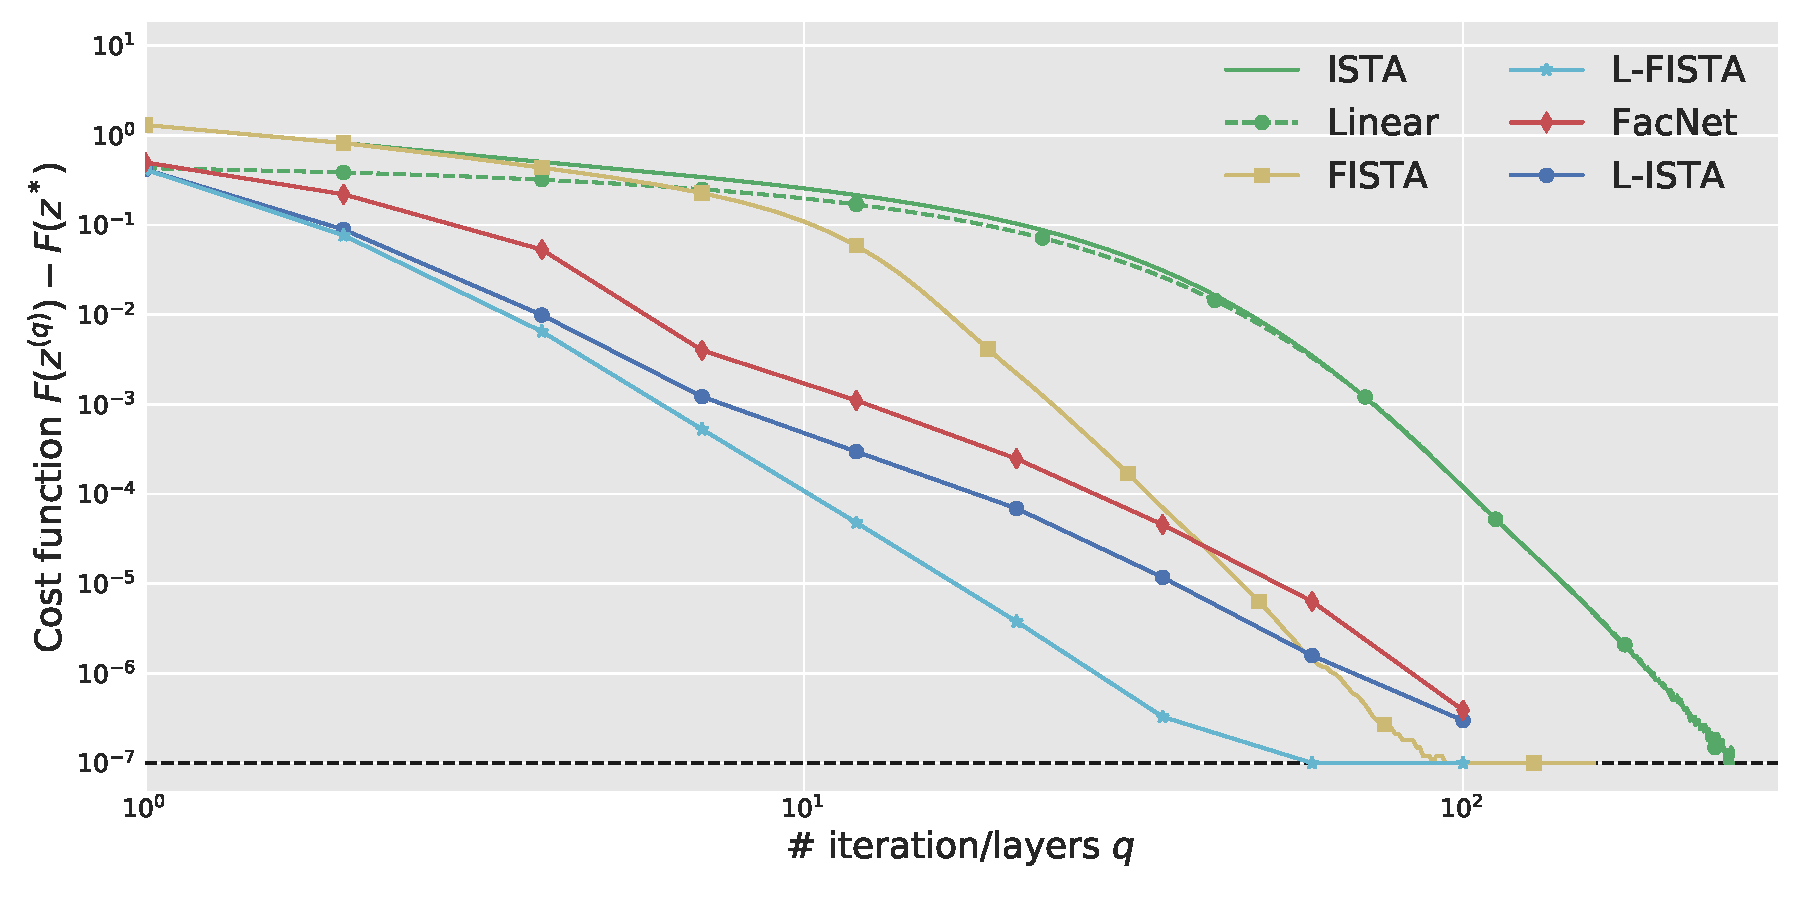
\includegraphics[width=.8\textwidth]{curve_sparse005_seaborn}\\
    Evolution of the cost function $F(z^{(q)}) - F(z^*)$ with the number of layers/iterations $q$ with a sparse model $\rho = {}^1/_{20}$.
\end{frame}

\begin{frame}[noframenumbering]{Artificial simulation}
\centering
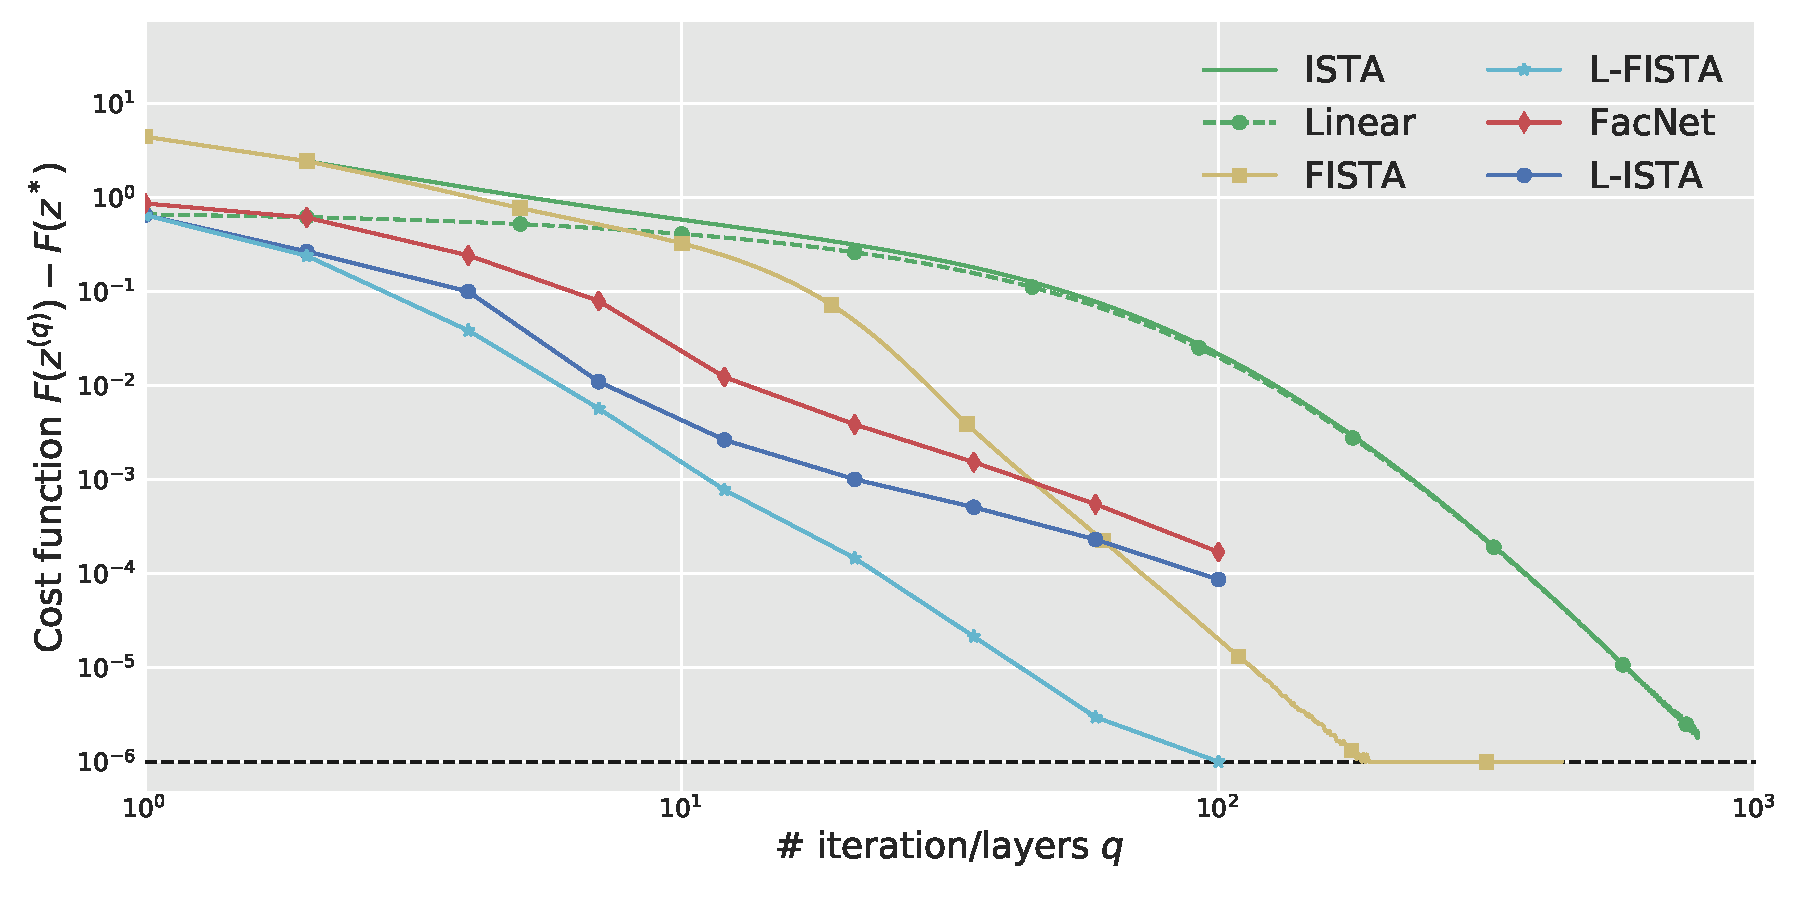
\includegraphics[width=.8\textwidth]{curve_sparse02_seaborn}\\
    Evolution of the cost function $F(z^{(q)}) - F(z^*)$ with the number of layers/iterations $q$ with a denser model $\rho = {}^1/_{4}$.
\end{frame}


\begin{frame}{Adversarial dictionary}

	\begin{columns}[T]
		\column{.35\textwidth}
		{\bf Adversarial dictionary:}\\
		$D = \begin{bmatrix} d_1 \dots d_K \end{bmatrix} \in \Rset^{K\times p}~,$ with 
		\[
			d_j = e^{-i \frac{2\pi j \zeta_q}{K}}
		\]
		for a random subset of frequencies $\left \{ \zeta_i \right \}_{i \le m}$ 
			
		\column{.65\textwidth}
		\includegraphics[width=\textwidth]{dictionary}
	\end{columns}
	\vskip2em
	\hskip2em $\Rightarrow$ Eigenvectors of $D$ are far from canonical basis.
\end{frame}


\begin{frame}[noframenumbering]{Adversarial dictionary}
\centering
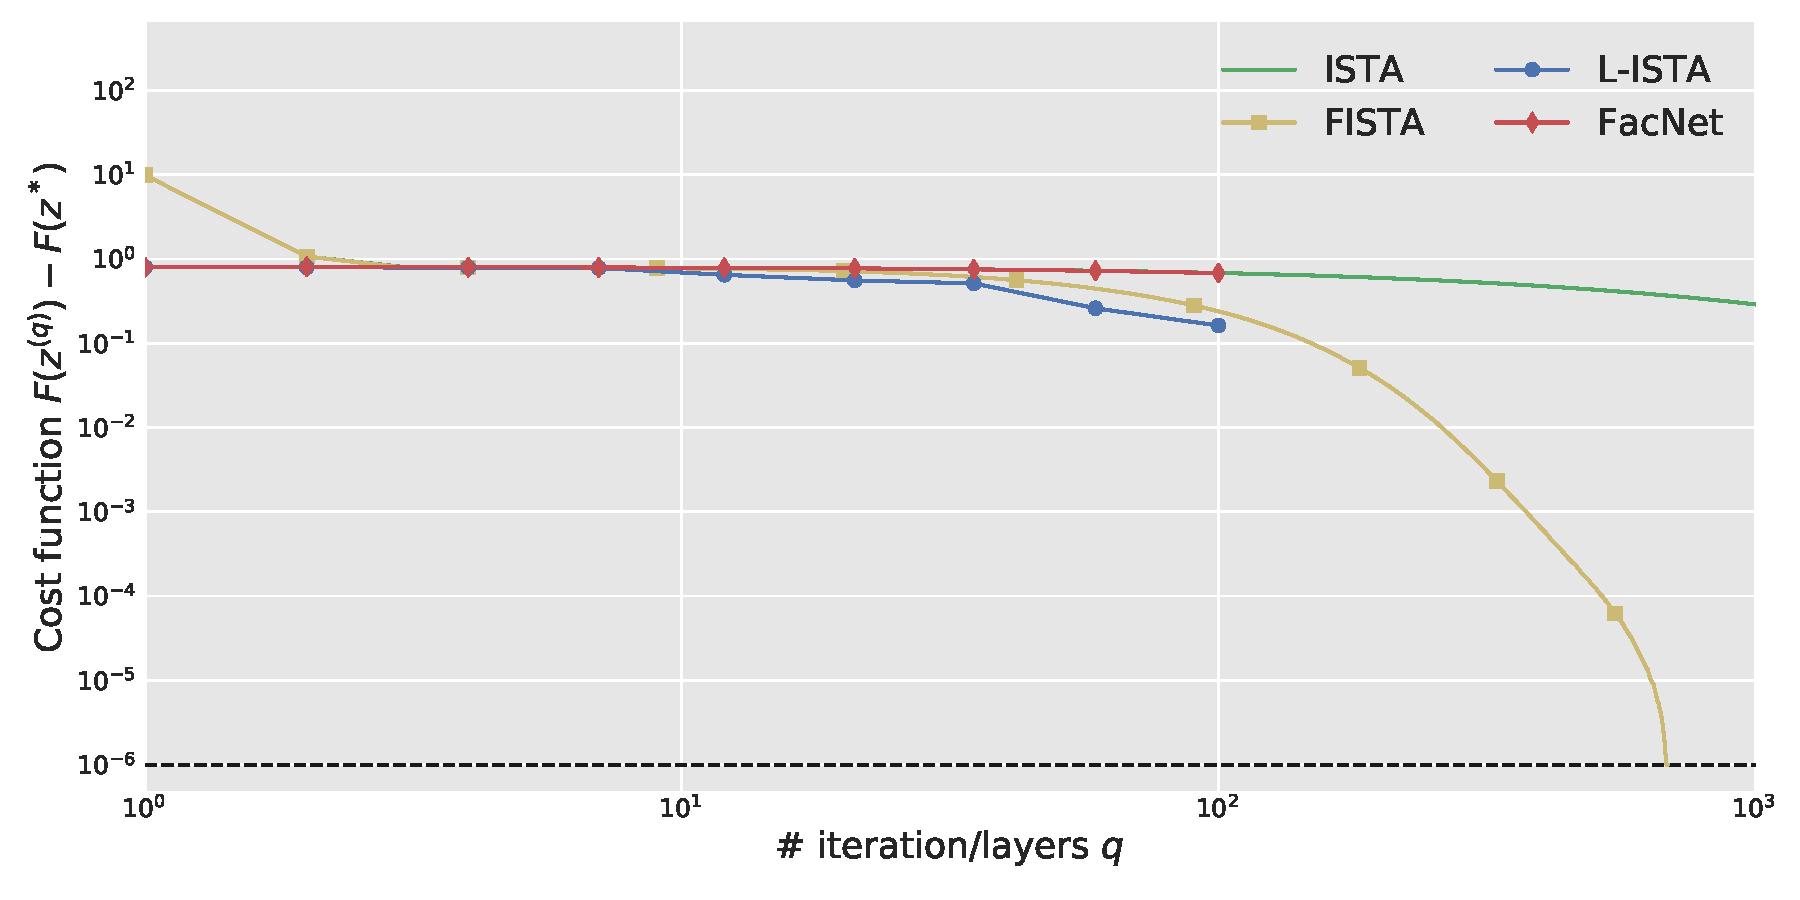
\includegraphics[width=.8\textwidth]{curve_adverse_seaborn}\\
    Evolution of the cost function $F(z^{(q)}) - F(z^*)$ with the number of layers/iterations k with n adversarial dictionary.
\end{frame}

\begin{frame}{PASCAL 08}

\begin{columns}[T]
\column{.49\textwidth}
\vskip2em
Sparse coding for the PASCAL 08 datasets over the Haar wavelets family.\\[2em]

The sparse coding is performed for patches of size $8\times8$.\\[.5em]
Train over 500 images and test over 100 images.
\column{.49\textwidth}
\includegraphics[width=\textwidth]{Wavlets}
	
\end{columns}
	
\end{frame}
\begin{frame}[noframenumbering]{PASCAL 08}
    \centering
    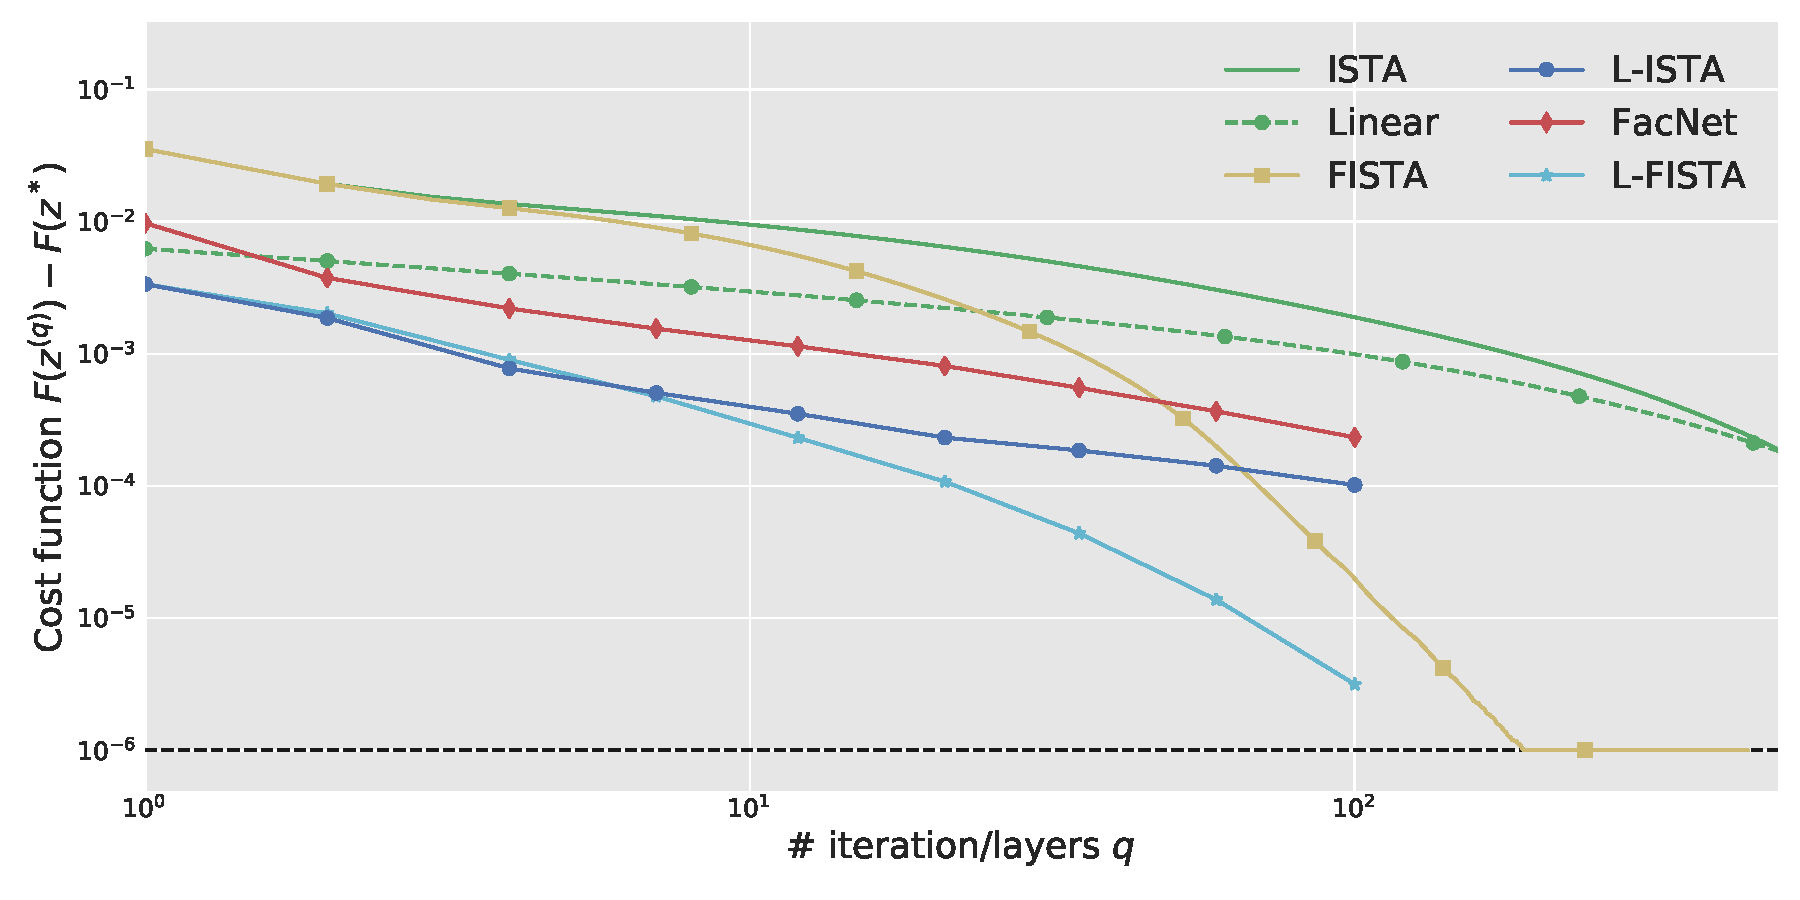
\includegraphics[width=.8\textwidth]{curve_images_seaborn}\\
     Evolution of the cost function $F(z^{(q)})-F(z^*)$ with the number of layers or the number of iteration $q$ for Pascal VOC 2008.
\end{frame}


\begin{frame}{MNIST}
	Dictionary $D$ with $K=100$ atoms learned on 10 000 MNIST samples (17x17) with dictionary learning.
	LISTA trained with MNIST training set and tested on MNIST test set.

    \centering
    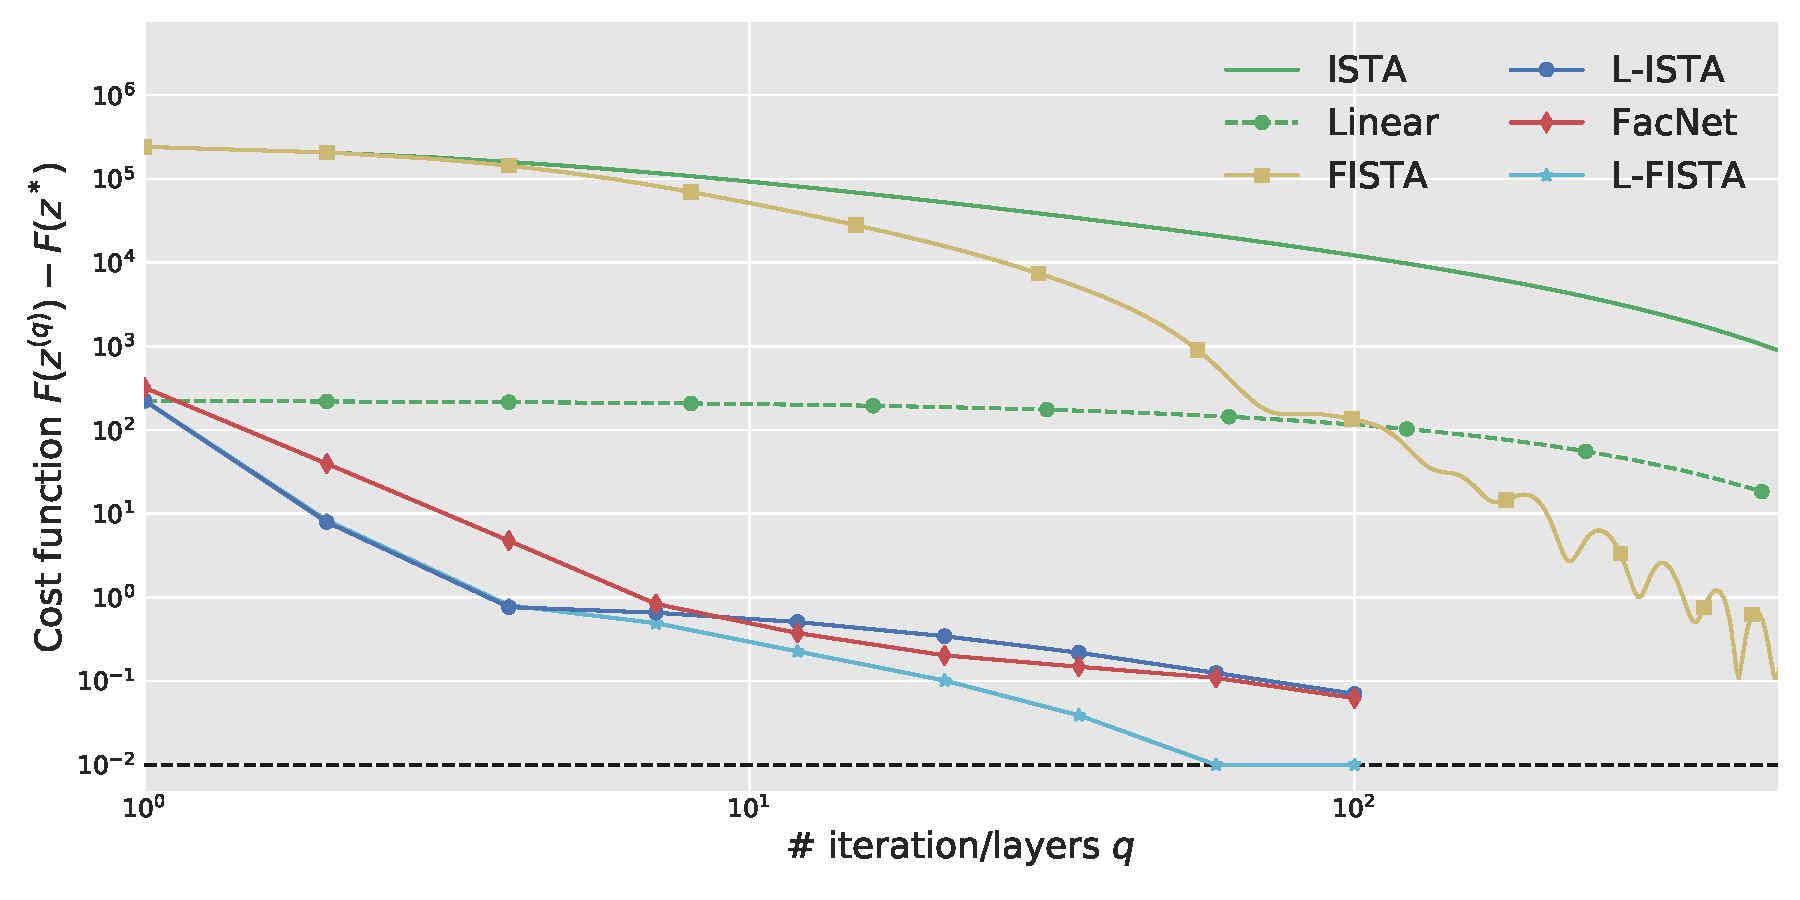
\includegraphics[width=.8\textwidth]{curve_mnist_seaborn}\\
     Evolution of the cost function $F(z^{(q)})-F(z^*)$ with the number of layers or the number of iteration $q$ for MNIST.
\end{frame}

\begin{frame}{Conclusion}
\begin{itemize}\itemsep1.5em
	\item Non asymptotic acceleration is possible :\\
	Approximate matrix factorization of $B=D\tran D$
	\begin{itemize}
	    \item Nearly diagonalize the kernel,
	    \item $\ell_1$-norm nearly invariant by this orthogonal transformation.
    \end{itemize}

    \item \emph{Future work:}
    \begin{itemize}
	    \item Improve the factorization formulation:
	    
	    \[ 
	    	\min_{A\tran A= \pmb I_K} f(\|DA\|_{1, 2}) + \lambda_q\frac{\|A\|_{1,1}}{n}~,
	    \]
	    \item Give generic bounds for sub gaussian $D$,
	    \item Link to Sparse PCA.
    \end{itemize}
\end{itemize}
	
\end{frame}


\begin{frame}{Conclusion}

	\vskip4em
	\begin{center}
		\Huge
		\textbf{Questions?}
	\end{center}
	
	\Large\vskip2em
	\begin{itemize}
	\item[] Code: \link{tomMoral/AdaptiveOptim}{github} 
	\item[] Paper: \url{https://arxiv.org/abs/1706.01338}\\[1em]
	\end{itemize}
	\vskip2em
	More at
	 \link[https://tommoral.github.io]{tommoral.github.io}{website}
	 \link[https://github.com/tomMoral]{tomMoral}{github}
\end{frame}



%-----------------------------------------------------------------------------
% References
%-----------------------------------------------------------------------------
{
\setbeamertemplate{footline}{} 
\begin{frame}{References}
	%\nocite{*}
	\tiny \bibliography{library.bib}
\end{frame}
}

\end{document} 